
\chapter{The distributive property}

The distributive law will be the star of this show.  What does this require?
\begin{align}
    u*(v+\acute{v}) & = u*v+u*\acute{v}
    & 
    (u+\acute{u})*v & = u*v + \acute{u}*v.
\end{align}
We definitely need additions, but we should not jump to assume that $u$, $v$, and $w$ are 
of the same type.  Just look at  matrix 
multiplication (we use $\mathbb{R}^{a\times b}$ to denote $(a\times b)$-matrices 
of real numbers)
\begin{align*}
    *&:\mathbb{R}^{a\times b}\times \mathbb{R}^{b\times c}\to \mathbb{R}^{a\times c}
    &
    (u*v)_{ij} & = \sum_k u_{ik}v_{kj}.
\end{align*}
So we except this is a study of \emph{heterogeneous} algebra, so we wont be
captivated by homomorphism but rather what we will call \emph{hetero}morphisms.
So we could think of three types of data $U$, $V$ and $W$ each with a $+$ each
combined by a function 
$*:U\times V\to W$
that satisfies the distributive law.  Because this is the start it will get its own 
notation, we write $\bmto$, that is 
\begin{align*}
    *:U\times V\bmto W
\end{align*}
denotes a distributive function on additive structures $U$, $V$, and $W$.
As we go along we will prefer to use $U$, $V$ and $W$ in just this way so that 
we can get up to speed on examples as quickly as possible.


\section{Properties of addition}
It is tempting now to start  assuming that $U$, $V$, and $W$ are 
something family---vector spaces, modules, or at least abelian groups.
However this would rob the distributive law of its power and leave us to think 
addition and its common attributes are the reason tensors work.  But the 
distributive law is already claiming a strong interaction of two operations 
so maybe it should be explored on its own a little while longer to appreciate 
what it already says about the individual operations.  More examples will demonstrate 
the value of a general point of view.

We will use a number of spaces
\begin{align*}
    \mathbb{R}^d & \defeq \{u:[d]\to \mathbb{R}\},\\
    R^{m\times n} &\defeq \{M:[m]\times [n]\to \mathbb{R}\}\\
    R^{\ell\times m\times n} &\defeq \{\Gamma:[\ell]\times [m]\times [n]\to \mathbb{R}\}\\
    & \vdots
\end{align*}
Define the following operations.
\begin{gather*}
    \mathbb{R}^m\oplus \mathbb{R}^n  \defeq \mathbb{R}^{m+n}\\
    \begin{bmatrix} \mathbb{R}^{a\times n} \\ \mathbb{R}^{b\times n} \end{bmatrix} \defeq \mathbb{R}^{(a+b)\times n}
    \qquad
    \begin{bmatrix}
    \mathbb{R}^{m\times c} &
    \mathbb{R}^{m\times d}
    \end{bmatrix}  \defeq \mathbb{R}^{m\times (c+d)}\\
%     \mathbb{R}^{a\times m\times n} \oplus \mathbb{R}^{b\times m\times n}  \defeq \mathbb{R}^{(a+b)\times m\times n}
%     \qquad
%     \mathbb{R}^{\ell \times c\times n} \oplus \mathbb{R}^{\ell \times d\times n}  \defeq \mathbb{R}^{\ell\times (c+d)\times n}
%     \qquad
% \\  
%      \mathbb{R}^{\ell \times m\times e} \oplus \mathbb{R}^{\ell \times m\times f}  \defeq \mathbb{R}^{\ell\times m\times (e+f)}\\
     \vdots
\end{gather*}

Now we add a multiplication.
\begin{align*}
    \mathbb{R}^m \otimes \mathbb{R}^n & \defeq \mathbb{R}^{m\times n}
\end{align*}

\begin{example}
    The distributive law with vector space operators.
    \begin{align*}
    (\mathbb{R}^a \oplus \mathbb{R}^b)\otimes \mathbb{R}^n 
        % & = \mathbb{R}^{(a+b)\times c}
        &  = \begin{bmatrix}\mathbb{R}^{a}\otimes \mathbb{R}^n  \\ \mathbb{R}^b\otimes \mathbb{R}^n\end{bmatrix}\\
    \mathbb{R}^m\oplus ( \mathbb{R}^c \oplus \mathbb{R}^d )
        % & = \mathbb{R}^{(a+b)\times c}
        &  = \begin{bmatrix} 
            \mathbb{R}^{m}\otimes \mathbb{R}^c &
            \mathbb{R}^m\otimes \mathbb{R}^d
        \end{bmatrix}
    \end{align*}
\end{example}

Lets combine the left and right 
distributive laws.

\begin{center}
    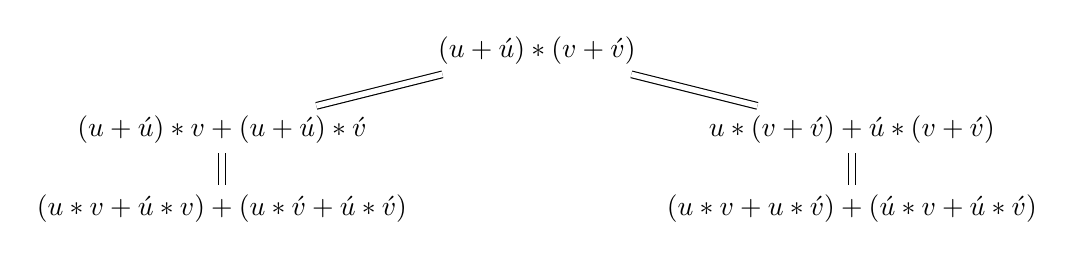
\begin{tikzpicture}[xscale=2]
        \node (A) at (0,0) {$(u+\acute{u})*(v+\acute{v})$};
        \node (B) at (-2,-1) {$(u+\acute{u})*v+(u+\acute{u})*\acute{v}$};
        \node (C) at (2,-1) {$u*(v+\acute{v})+\acute{u}*(v+\acute{v})$};
        \node (D) at (-2,-2) {$(u*v+\acute{u}*v)+(u*\acute{v}+\acute{u}*\acute{v})$};
        \node (E) at (2,-2) {$(u*v+u*\acute{v})+(\acute{u}*v+\acute{u}*\acute{v})$};
        \draw[double distance=2pt] (A) -- (B);
        \draw[double distance=2pt] (A) -- (C);
        \draw[double distance=2pt] (B) -- (D);
        \draw[double distance=2pt] (C) -- (E);
    \end{tikzpicture}
\end{center}
Thus the values $a,b,c,d,\ldots $ in the image of a distributive product $*:U\times V\bmto W$ must 
satisfy the following identity.
\begin{equation}
    \tag{Distributable}
    (a+b)+(c+d) = (a+c)+(b+d)
\end{equation}

\begin{proposition}
    If $+$ in both associative and commutative then it is distributable.

    Conversely, if $+$ is 
\end{proposition}